\chapter{จุลชีววิทยาในระบบปศุสัตว์ กระเพาะรูเมน และเพาะเลี้ยงสัตว์น้ำ}
\label{ch:animal_husbandry}

\begin{keyconcept}[แนวคิดสำคัญของบทที่ 7]
ระบบนิเวศจุลินทรีย์ในทางเดินอาหารของสัตว์และแหล่งน้ำเพาะเลี้ยงมีความสัมพันธ์อย่างแนบแน่นต่อสุขภาพ ผลผลิต และผลกระทบต่อสิ่งแวดล้อม ในสัตว์เคี้ยวเอื้อง กระเพาะรูเมน (Rumen)\index{จุลชีววิทยาในกระเพาะรูเมน (Rumen Microbiology)} ทำหน้าที่เสมือนถังหมักไร้ออกซิเจนแบบธรรมชาติที่จุลินทรีย์หลายพันสายพันธุ์ทำงานประสานกันเพื่อย่อยสลายเซลลูโลสเป็นกรดไขมันระเหยง่าย (VFAs)\index{กรดไขมันระเหยง่าย (Volatile Fatty Acids: VFAs)} ที่เป็นแหล่งพลังงานหลักของสัตว์ ควบคู่ไปกับกระบวนการสร้างก๊าซมีเทนโดยอาร์เคีย\index{กระบวนการสร้างมีเทน (Methanogenesis)} สำหรับภาคการเพาะเลี้ยงสัตว์น้ำหนาแน่นสูง การควบคุมวงจรไนโตรเจน การบำบัดแอมโมเนียด้วยเทคโนโลยีไบโอฟล็อก (Biofloc Technology: BFT)\index{เทคโนโลยีไบโอฟล็อก (Biofloc Technology: BFT)} และการใช้จุลินทรีย์โพรไบโอติกเพื่อยับยั้งสารพิษ PirA/PirB\index{สารพิษไบนารี PirA/PirB} ของแบคทีเรีย \organism{Vibrio parahaemolyticus}\index{Vibrio parahaemolyticus@\textit{Vibrio parahaemolyticus}} ก่อโรคตายด่วนในกุ้ง (AHPND)\index{โรคตายด่วนในกุ้ง (AHPND/EMS)} ถือเป็นกุญแจสำคัญสู่ความยั่งยืนของการเพาะเลี้ยงสัตว์น้ำสมัยใหม่
\end{keyconcept}

\begin{figure}[ht]
    \centering
    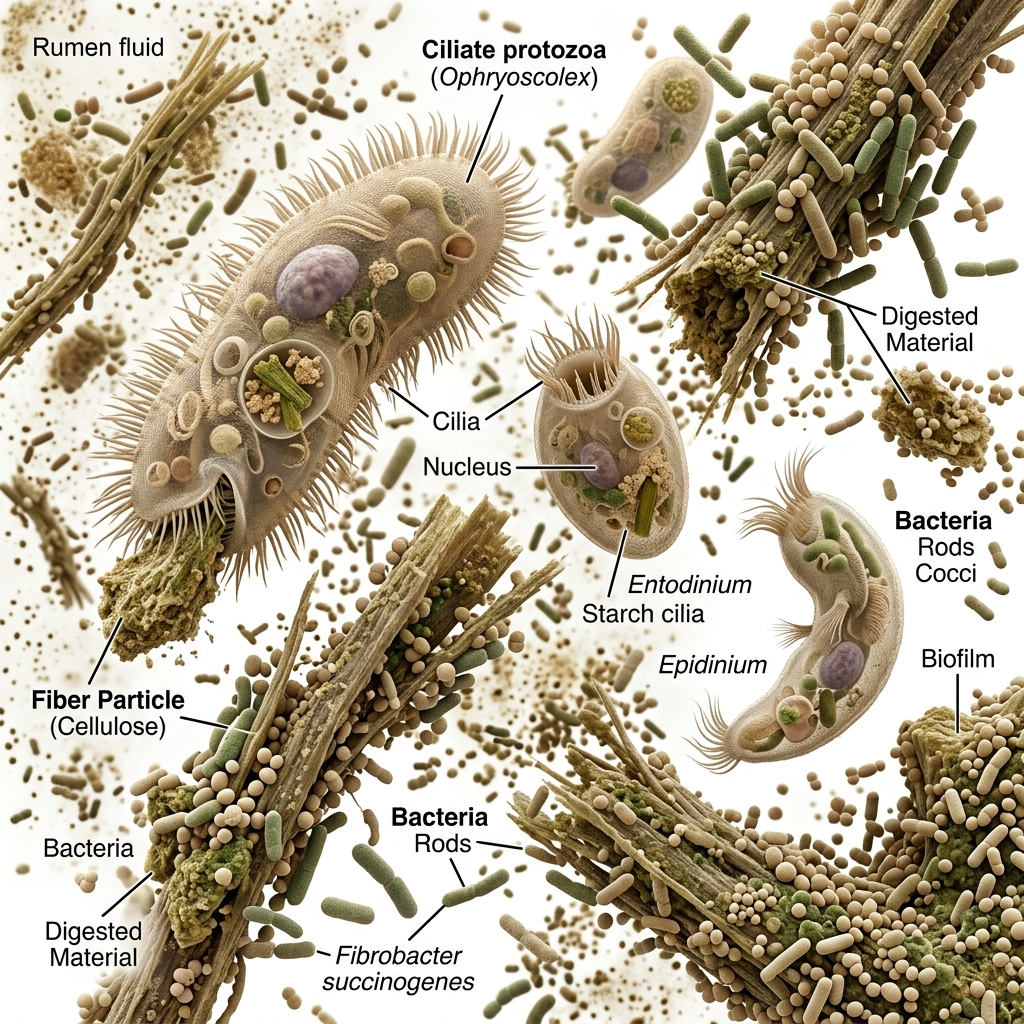
\includegraphics[width=0.85\textwidth]{assets/ch07_rumen_microbes.png}
    \caption{การจำลอง 3D ของระบบนิเวศในรูเมน (Rumen ecosystem) แสดงปฏิสัมพันธ์ระหว่างแบคทีเรียย่อยเยื่อใยพืช โปรโตซัวกลุ่มมีซิเลีย (Ciliates) เส้นใยเชื้อรากระเพาะหมัก (\organism{Neocallimastix}) และกลุ่มอาร์เคียสร้างก๊าซมีเทน (Methanogenic Archaea) ที่เกาะติดและย่อยสลายผนังเซลล์พืชในสภาวะแอนแอโรบิกอย่างสมบูรณ์}
    \label{fig:ch07_rumen_microbes}
\end{figure}

\section*{วัตถุประสงค์การเรียนรู้ประจำบท}
เมื่อศึกษาบทเรียนนี้จบแล้ว นักศึกษาสามารถ:
\begin{enumerate}
    \item อธิบายสรีรวิทยาสภาพแวดล้อมและโครงสร้างความหลากหลายของจุลินทรีย์ในกระเพาะรูเมน (แบคทีเรีย โปรโตซัว รา และอาร์เคีย)
    \item เขียนสมการสโตอิชิโอเมตรีการหมักคาร์โบไฮเดรตในรูเมนเป็นกรดไขมันระเหยง่าย (Acetate, Propionate, Butyrate) และการสร้างก๊าซมีเทน
    \item วิเคราะห์แนวทางการลดการปล่อยก๊าซมีเทนจากสัตว์เคี้ยวเอื้องด้วยสารยับยั้งจำเพาะและโภชนศาสตร์จุลินทรีย์
    \item อธิบายกลไกการเปลี่ยนรูปของเสียไนโตรเจน (TAN $\rightarrow NO_2^- \rightarrow NO_3^-$) และคำนวณการปรับสมดุล C:N Ratio ในระบบไบโอฟล็อก (Biofloc)
    \item วิเคราะห์พยาธิกำเนิดของสารพิษไบนารีท็อกซิน PirA/PirB จากเชื้อ \organism{Vibrio parahaemolyticus} (AHPND) ในกุ้ง และกลไกของโพรไบโอติกในการควบคุมโรค
\end{enumerate}

\section{ระบบนิเวศสรีรวิทยาและสังคมจุลินทรีย์ในกระเพาะรูเมน}

กระเพาะรูเมน (Rumen) ของสัตว์เคี้ยวเอื้อง (โค กระบือ แพะ แกะ) เป็นเครื่องปฏิกรณ์ชีวภาพแบบหมักต่อเนื่องไร้ออกซิเจนขนาดใหญ่ โดยในโคนมโตเต็มวัยมีปริมาตรจุสารหมักได้ถึง $100 - 250\text{ ลิตร}$ สภาพแวดล้อมภายในรูเมนถูกควบคุมอย่างจำเพาะสูง:
\begin{itemize}
    \item \textbf{อุณหภูมิคงที่:} $38.5 - 40.0^\circ\text{C}$
    \item \textbf{ความเป็นกรด-ด่าง (pH):} $5.8 - 6.8$ (ควบคุมด้วยน้ำลายที่มีสารบัฟเฟอร์ไบคาร์บอเนตและฟอสเฟตสูงถึง 150 ลิตรต่อวัน)
    \item \textbf{ศักย์ออกซิเดชัน-รีดักชัน (Redox Potential: $E_h$):} ต่ำกว่า $-350\text{ mV}$ (สภาวะแอนแอโรบิกเข้มงวด)
\end{itemize}

\subsection{องค์ประกอบของสังคมจุลินทรีย์ในรูเมน}
\begin{enumerate}
    \item \textbf{แบคทีเรียในรูเมน (Rumen Bacteria, $10^{10} - 10^{11}\text{ เซลล์/mL}$):}
    \begin{itemize}
        \item \textit{กลุ่มย่อยเซลลูโลสและเฮมิเซลลูโลส (Fibrolytic):} \organism{Fibrobacter succinogenes}\index{Fibrobacter succinogenes@\textit{Fibrobacter succinogenes}}, \organism{Ruminococcus albus}\index{Ruminococcus albus@\textit{Ruminococcus albus}}, และ \organism{Ruminococcus flavefaciens} สร้างเอนไซม์ Cellulase และ Xylanase ย่อยสลายโครงสร้างผนังเซลล์พืช
        \item \textit{กลุ่มย่อยแป้งและน้ำตาล (Amylolytic):} \organism{Streptococcus bovis}\index{Streptococcus bovis@\textit{Streptococcus bovis}}, \organism{Ruminobacter amylophilus}, และ \organism{Succinimonas amylolytica}
        \item \textit{กลุ่มใช้น้ำตาลและกรดแลกติก (Acid-utilizing):} \organism{Megasphaera elsdenii}\index{Megasphaera elsdenii@\textit{Megasphaera elsdenii}} และ \organism{Selenomonas ruminantium} ช่วยเปลี่ยนกรดแลกติกเป็นกรดโพรพิโอนิก ป้องกันภาวะกรดเกินในรูเมน (Acidosis)
    \end{itemize}
    \item \textbf{โปรโตซัวในรูเมน (Rumen Protozoa, $10^5 - 10^6\text{ เซลล์/mL}$):} ส่วนใหญ่เป็นซิลิเอต (Ciliates) เช่น \organism{Entodinium}, \organism{Epidinium}, และ \organism{Polyplastron} ทำหน้าที่กลืนกินเม็ดแป้งอย่างรวดเร็วเพื่อชะลออัตราการหมัก และล่ากินแบคทีเรียเพื่อหมุนเวียนโปรตีน
    \item \textbf{เชื้อราในรูเมน (Anaerobic Gut Fungi, $10^3 - 10^5\text{ ซูโอสปอร์/mL}$):} เช่น สกุล \organism{Neocallimastix}\index{Neocallimastix@\textit{Neocallimastix}}, \organism{Piromyces}, และ \organism{Orpinomyces} เส้นใยไรซอยด์ (Rhizoids) สามารถแทงทะลุเปลือกชั้นลิกนินที่แข็งกระด้างของพืช เปิดทางให้แบคทีเรียแทรกเข้าไปย่อยเนื้อเยื่อภายใน
    \item \textbf{อาร์เคียสร้างมีเทน (Methanogenic Archaea, $10^8 - 10^9\text{ เซลล์/mL}$):} เช่น \organism{Methanobrevibacter ruminantium}\index{Methanobrevibacter ruminantium@\textit{Methanobrevibacter ruminantium}} และ \organism{Methanosphaera stadtmanae} ใช้อิเล็กตรอนและไฮโดรเจนอิสระ ($H_2$) รีดิวซ์คาร์บอนไดออกไซด์เป็นก๊าซมีเทน
\end{enumerate}

\section{สโตอิชิโอเมตรีของการหมักกรดไขมันระเหยง่ายและการสร้างมีเทน}

การย่อยสลายพอลิแซ็กคาไรด์ในรูเมนผ่านกระบวนการไกลโคไลซิสจะได้โมเลกุลน้ำตาลเฮกโซส (Hexose: กลูโคส) จากนั้นถูกหมักผ่านวิถีชีวเคมีต่างๆ เกิดเป็นกรดไขมันระเหยง่าย (Volatile Fatty Acids: VFAs)\index{กรดไขมันระเหยง่าย (Volatile Fatty Acids: VFAs)} 3 ชนิดหลัก:

\subsection{1. ปฏิกิริยาสังเคราะห์กรดอะซิติก (Acetate Pathway)}
\begin{equation}
C_6H_{12}O_6 + 2 H_2O \longrightarrow 2 CH_3COOH + 2 CO_2 + 4 H_2
\end{equation}
ปฏิกิริยานี้ปลดปล่อยก๊าซไฮโดรเจนอิสระออกมามาก ($4\text{ โมล } H_2\text{ ต่อโมลกลูโคส}$) สัตว์นำอะซิเตตไปใช้สังเคราะห์ไขมันในเนื้อเยื่อและไขมันในน้ำนม (Milk fat)\index{กรดอะซิติก (Acetate)}

\subsection{2. ปฏิกิริยาสังเคราะห์กรดบิวไทริก (Butyrate Pathway)}
\begin{equation}
C_6H_{12}O_6 \longrightarrow CH_3CH_2CH_2COOH + 2 CO_2 + 2 H_2
\end{equation}
ปลดปล่อยก๊าซไฮโดรเจน $2\text{ โมล } H_2$ สัตว์นำบิวไทเรตไปใช้เป็นพลังงานของเซลล์บุผนังกระเพาะรูเมน (Rumen papillae)\index{กรดบิวไทริก (Butyrate)}

\subsection{3. ปฏิกิริยาสังเคราะห์กรดโพรพิโอนิก (Propionate Pathway)}
ดำเนินผ่านวิถีซักซิเนต (Succinate pathway) หรือวิถีอะคริเลต (Acrylate pathway):\index{กรดโพรพิโอนิก (Propionate)}
\begin{equation}
C_6H_{12}O_6 + 2 H_2 \longrightarrow 2 CH_3CH_2COOH + 2 H_2O
\end{equation}
ปฏิกิริยานี้ **บริโภคไฮโดรเจนอิสระ ($2\text{ โมล } H_2$)** เข้าไปในโมเลกุล กรดโพรพิโอเนตจะถูกดูดซึมส่งไปยังตับเพื่อสังเคราะห์เป็นน้ำตาลกลูโคส (Gluconeogenesis) ซึ่งเป็นแหล่งพลังงานหลักของร่างกายและการเจริญเติบโต

\subsection{4. กระบวนการสร้างก๊าซมีเทน (Methanogenesis) และการควบคุม}
ก๊าซไฮโดรเจน ($H_2$) ที่เกิดขึ้นจากวิถีอะซิเตตและบิวไทเรต หากสะสมมากเกินไปจะยับยั้งเอนไซม์ดีไฮโดรจีเนสและหยุดการทำงานของจุลินทรีย์ทั้งระบบ อาร์เคียสร้างมีเทนจึงทำหน้าที่เป็นถังรับไฮโดรเจน (Hydrogen sink):
\begin{equation}
CO_2 + 4 H_2 \longrightarrow CH_4 + 2 H_2O \quad (\Delta G^\circ = -131\text{ kJ/mol})
\end{equation}
อย่างไรก็ดี ก๊าซมีเทนที่สัตว์เรอออกมาคิดเป็นการสูญเสียพลังงานของอาหารสัตว์ถึงร้อยละ 6--12 และเป็นก๊าซเรือนกระจกที่มีศักยภาพโลกร้อนสูงกว่า $CO_2$ ถึง 28 เท่า ในปัจจุบันมีการใช้สารยับยั้งทางชีวเคมี เช่น สารสกัดสาหร่ายสีแดง (\organism{Asparagopsis taxiformis}) ซึ่งมีสารโบรโมฟอร์ม (Bromoform) หรือสาร 3-Nitrooxypropanol (3-NOP) ยับยั้งเอนไซม์ Methyl-coenzyme M reductase (MCR) ช่วยลดการปล่อยมีเทนได้มากกว่า $30 - 80\%$

\section{จุลชีววิทยาทางเพาะเลี้ยงสัตว์น้ำและวงจรไนโตรเจน}

ในการเพาะเลี้ยงกุ้งและปลาหนาแน่นสูง อาหารเม็ดโปรตีนสูงที่สัตว์กินและขับถ่ายออกมารวมทั้งอาหารที่เหลือตกค้าง จะสลายตัวกลายเป็น \textbf{ไนโตรเจนแอมโมเนียรวม (Total Ammonia Nitrogen: TAN)\index{แอมโมเนียรวม (TAN: Total Ammonia Nitrogen)}}:

\begin{equation}
\text{TAN} = [NH_3] + [NH_4^+]
\end{equation}

สัดส่วนของแอมโมเนียอิสระไร้ประจุ ($NH_3$) ซึ่งมีความเป็นพิษสูงมากต่อเหงือกและระบบประสาทของสัตว์น้ำ จะแปรผันตามค่า pH และอุณหภูมิของน้ำ:

\begin{equation}
\% NH_3 = \frac{100}{1 + 10^{(pK_a - \text{pH})}}
\end{equation}

เมื่อ $pK_a \approx 9.24$ ที่อุณหภูมิ $28^\circ\text{C}$ หากน้ำในบ่อมีค่า $\text{pH } 8.5$ สัดส่วนของ $NH_3$ จะสูงถึงประมาณ $15\%$ ของ TAN ทั้งหมด ซึ่งเป็นอันตรายถึงชีวิตต่อสัตว์น้ำหาก TAN เกิน $1 - 2\text{ mg/L}$

\subsection{1. กระบวนการไนตริฟิเคชันแบบออโตโทรฟิก (Autotrophic Nitrification)}
ในระบบกรองชีวภาพ (Biofilter) แบคทีเรียไนตริฟายเออร์จะทำปฏิกิริยาออกซิเดชันสองขั้นตอน:
\begin{itemize}
    \item แอมโมเนียออกซิไดซิงแบคทีเรีย (AOB: เช่น \organism{Nitrosomonas}):
    $$2 NH_4^+ + 3 O_2 \longrightarrow 2 NO_2^- + 4 H^+ + 2 H_2O$$
    \item ไนไตรต์ออกซิไดซิงแบคทีเรีย (NOB: เช่น \organism{Nitrobacter}, \organism{Nitrospira}):
    $$2 NO_2^- + O_2 \longrightarrow 2 NO_3^-$$
\end{itemize}
กระบวนการนี้ต้องการออกซิเจนสูง ($4.57\text{ g } O_2$ ต่อน้ำหนัก $1\text{ g } NH_4^+$-N) และทำลายความเป็นด่าง (Alkalinity) ในน้ำ โดยกินด่างไปถึง $7.14\text{ g } CaCO_3$ ต่อน้ำหนัก $1\text{ g } NH_4^+$-N ผู้เลี้ยงจึงต้องเติมปูนขาวหรือโซเดียมไบคาร์บอเนตอย่างสม่ำเสมอ

\subsection{2. เทคโนโลยีไบโอฟล็อก (Biofloc Technology: BFT)}
แทนที่จะพึ่งพาแบคทีเรียออโตโทรฟที่เติบโตช้า ระบบ Biofloc\index{เทคโนโลยีไบโอฟล็อก (Biofloc Technology: BFT)} อาศัยการเติมนิ่งคาร์บอน (เช่น กากน้ำตาล รำข้าว แป้งมันสำปะหลัง) เพื่อปรับอัตราส่วนคาร์บอนต่อไนโตรเจน (\textbf{C:N Ratio $\ge 15:1$}\index{อัตราส่วน C:N (Carbon-to-Nitrogen Ratio)}):
\begin{itemize}
    \item แบคทีเรียกลุ่ม \textbf{Heterotrophic Bacteria\index{แบคทีเรียเฮเทอโรโทรฟิก (Heterotrophic Bacteria)}} จะใช้น้ำตาลเป็นแหล่งพลังงานและดูดซับแอมโมเนียมไอออน ($NH_4^+$) เข้าไปสังเคราะห์เป็นโปรตีนเซลล์จุลินทรีย์ (Single-Cell Protein) อย่างรวดเร็ว (เร็วกว่าไนตริฟิเคชัน 10 เท่า)
    \item แบคทีเรียจะสร้างสารพอลิเมอร์นอกเซลล์ (EPS) จับตัวกับแพลงก์ตอนพืชและโปรโตซัว รวมกันเป็นตะกอนแขวนลอยเรียกว่า \textbf{ก้อนฟล็อก (Biofloc)}
    \item กุ้งและปลาสามารถตอดกินก้อนฟล็อกเป็นอาหารโปรตีนธรรมชาติ (มีโปรตีน $25 - 35\%$) ช่วยลดอัตราการใช้อาหารเม็ด (FCR) และลดการเปลี่ยนถ่ายน้ำสู่สิ่งแวดล้อมภายนอกได้เกือบ $100\%$
\end{itemize}

\begin{figure}[ht]
\centering
\begin{tikzpicture}[
    scale=0.88, every node/.style={scale=0.88},
    box/.style={draw=navyprimary, fill=white, rounded corners=5pt, text width=3.4cm, align=center, line width=1pt},
    patha/.style={draw=blue!80!black, fill=blue!8, rounded corners=5pt, text width=3.3cm, align=center, line width=1pt},
    pathb/.style={draw=forestgreen, fill=forestgreen!10, rounded corners=5pt, text width=3.3cm, align=center, line width=1pt},
    arrow/.style={->, >=Stealth, line width=1.3pt}
]
    % Central source
    \node [box, fill=amber!15] (source) at (6, 4.5) {
        \textbf{ไนโตรเจนแอมโมเนียรวม}\\\textbf{(TAN: $NH_3 / NH_4^+$)}\\[2pt]
        {\scriptsize จากอาหารตกค้างและการขับถ่าย}
    };

    % Pathway A: Autotrophic Nitrification
    \node [patha] (nit1) at (2.2, 2.5) {
        \textbf{1. ไนไตรต์ ($NO_2^-$)}\\[2pt]
        {\scriptsize ออกซิไดซ์โดย AOB\\(\organism{Nitrosomonas})}
    };
    \node [patha] (nit2) at (2.2, 0.5) {
        \textbf{2. ไนเตรต ($NO_3^-$)}\\[2pt]
        {\scriptsize ออกซิไดซ์โดย NOB\\(\organism{Nitrobacter})}
    };
    \node [patha, fill=blue!15] (nita_sum) at (2.2, -1.5) {
        \textbf{ระบบไนตริฟิเคชันดั้งเดิม}\\[2pt]
        {\scriptsize $\bullet$ สิ้นเปลือง $O_2$ สูง\\$\bullet$ กินด่าง $7.14\text{ g } CaCO_3/\text{g N}$\\$\bullet$ ต้องถ่ายน้ำระบาย $NO_3^-$}
    };

    % Pathway B: Heterotrophic Biofloc
    \node [pathb] (bio1) at (9.8, 2.5) {
        \textbf{1. เติมคาร์บอน (C:N $\ge$ 15)}\\[2pt]
        {\scriptsize กากน้ำตาล / รำข้าว / แป้ง}
    };
    \node [pathb] (bio2) at (9.8, 0.5) {
        \textbf{2. การดูดซึมเร็ว}\\[2pt]
        {\scriptsize แบคทีเรีย Heterotrophs\\สังเคราะห์โปรตีนเซลล์}
    };
    \node [pathb, fill=forestgreen!20] (biob_sum) at (9.8, -1.5) {
        \textbf{ก้อนฟล็อกโปรตีน (Biofloc)}\\[2pt]
        {\scriptsize $\bullet$ กุ้ง/ปลาตอดกิน (ลด FCR)\\$\bullet$ ไม่ต้องเปลี่ยนถ่ายน้ำ ($0\%$)\\$\bullet$ กำจัด TAN เร็วกว่า 10 เท่า}
    };

    % Arrows Pathway A
    \draw [arrow, blue!80!black] (source) -| (nit1) node[midway, above left, font=\scriptsize] {Autotrophic};
    \draw [arrow, blue!80!black] (nit1) -- (nit2) node[midway, right, font=\scriptsize] {$+ O_2$};
    \draw [arrow, blue!80!black] (nit2) -- (nita_sum);

    % Arrows Pathway B
    \draw [arrow, forestgreen] (source) -| (bio1) node[midway, above right, font=\scriptsize] {Heterotrophic};
    \draw [arrow, forestgreen] (bio1) -- (bio2) node[midway, right, font=\scriptsize] {$+ NH_4^+$};
    \draw [arrow, forestgreen] (bio2) -- (biob_sum);

\end{tikzpicture}
\caption{การเปรียบเทียบพลวัตการกำจัดไนโตรเจนแอมโมเนียในบ่อเพาะเลี้ยงสัตว์น้ำ: ระบบกรองชีวภาพแบบไนตริฟิเคชันดั้งเดิม (Autotrophic Nitrification) กับเทคโนโลยีไบโอฟล็อก (Heterotrophic Biofloc Technology: BFT)}
\label{fig:aquaculture_nitrogen_pathways}
\end{figure}

\section{โรคตายด่วนในกุ้ง (AHPND/EMS) และการใช้โพรไบโอติกควบคุม}

\subsection{1. ชีวโมเลกุลสารพิษ PirA/PirB ของเชื้อ Vibrio parahaemolyticus}
โรคตับวายเฉียบพลันในกุ้ง (Acute Hepatopancreatic Necrosis Disease: AHPND หรือ EMS) เกิดจากแบคทีเรีย \organism{Vibrio parahaemolyticus} สายพันธุ์ก่อโรคที่มีพลาสมิด pVA1 ขนาด $69 - 73\text{ kb}$ ซึ่งมียีนสร้างสารพิษไบนารีท็อกซิน **PirA$^{vp}$ ($13\text{ kDa}$)** และ **PirB$^{vp}$ ($50\text{ kDa}$)**:
\begin{itemize}
    \item สารพิษ PirA และ PirB รวมตัวกันเป็นสารเชิงซ้อน (Heterodimer complex) ซึ่งมีโครงสร้างคล้ายสารพิษฆ่าแมลง Pir toxin ของแบคทีเรีย \organism{Photorhabdus}
    \item โปรตีน PirB เข้าจับกับตัวรับบนเยื่อหุ้มเซลล์ของท่อน้ำดีและตับอ่อนของกุ้ง (Hepatopancreas) จากนั้นแทงสร้างรูรั่ว นำพา PirA เข้าสู่เซลล์
    \item เซลล์ท่อตับอ่อนหลุดลอก (Massive Sloughing) ส่งผลให้เนื้อเยื่อตับอ่อนฝ่อลีบ ซีดขาว และกุ้งตายเกลื่อนบ่อภายใน $10 - 35\text{ วัน}$ หลังปล่อยลูกกุ้ง
\end{itemize}

\subsection{2. กลไกการออกฤทธิ์ของโพรไบโอติกในระบบทางเดินอาหารสัตว์น้ำ}
การเสริมแบคทีเรียโพรไบโอติก เช่น \organism{Bacillus subtilis}, \organism{Bacillus licheniformis}, และ \organism{Lactobacillus plantarum} ในอาหารกุ้งช่วยต้านทานเชื้อ \organism{Vibrio} ผ่าน 3 กลไกหลัก:
\begin{enumerate}
    \item \textbf{Quorum Quenching:} แบคทีเรีย \organism{Bacillus} สังเคราะห์เอนไซม์ **AHL Lactonase** สลายโมเลกุลส่งสัญญาณสื่อสารระหว่างเซลล์ (Acyl-Homoserine Lactone: AHL) ของเชื้อ \organism{Vibrio} ทำให้เชื้อไม่สามารถรวมกลุ่มสั่งการหลั่งสารพิษ PirA/PirB ได้
    \item \textbf{Competitive Exclusion:} เข้ายึดเกาะตัวรับบนเยื่อบุลำไส้กุ้งและผลิตสารแบคเทอริโอซิน (Bacteriocins) ยับยั้งการเจริญเติบโตของเชื้อก่อโรค
    \item \textbf{การกระตุ้นภูมิคุ้มกันกุ้ง (ProPO System):} ผนังเซลล์ของโปรไบโอติก ($\beta$-glucans และ Lipopolysaccharides) กระตุ้นการทำงานของเอนไซม์ Prophenoloxidase (ProPO) ในเม็ดเลือดกุ้ง ช่วยสังเคราะห์เมลานินเข้าห่อหุ้มและทำลายเชื้อก่อโรค
\end{enumerate}

\begin{worked}[ตัวอย่างที่ 7.1 การคำนวณสัดส่วน VFAs และการปลดปล่อยพลังงานจากการหมักในรูเมน]
ในโคเนื้อที่กินหญ้าแห้งเป็นอาหารหลัก จุลินทรีย์ในรูเมนผลิตกรดไขมันระเหยง่ายด้วยอัตราส่วนโมลาร์ดังนี้:
$$\text{Acetate } (A) : \text{Propionate } (P) : \text{Butyrate } (B) = 65 : 20 : 15$$
หากการหมักเริ่มต้นจากโมเลกุลกลูโคส 100 โมล จงคำนวณปริมาณไฮโดรเจนอิสระ ($H_2$) สุทธิที่เกิดขึ้น และคำนวณปริมาณก๊าซมีเทน ($CH_4$) ที่ถูกสร้างขึ้นตามทฤษฎี

\textbf{วิธีทำ:}
1. จากสมการสโตอิชิโอเมตรี:
\begin{itemize}
    \item 1 โมล Glucose $\rightarrow$ 2 โมล Acetate $+ 4$ โมล $H_2$ $\implies$ ผลิต $H_2 = 2.0\text{ โมลต่อโมล Acetate}$
    \item 1 โมล Glucose $\rightarrow$ 1 โมล Butyrate $+ 2$ โมล $H_2$ $\implies$ ผลิต $H_2 = 2.0\text{ โมลต่อโมล Butyrate}$
    \item 1 โมล Glucose $+ 2$ โมล $H_2 \rightarrow$ 2 โมล Propionate $\implies$ บริโภค $H_2 = 1.0\text{ โมลต่อโมล Propionate}$
\end{itemize}

2. คำนวณสมดุล $H_2$ จากสัดส่วนโมลาร์ $65A : 20P : 15B$:
$$H_{2\text{ สร้างขึ้น}} = (65 \times 2.0) + (15 \times 2.0) = 130 + 30 = 160\text{ โมล } H_2$$
$$H_{2\text{ บริโภค}} = 20 \times 1.0 = 20\text{ โมล } H_2$$
$$H_{2\text{ สุทธิ}} = 160 - 20 = 140\text{ โมล } H_2$$

3. คำนวณปริมาณมีเทน ($CH_4$) จากสมการ $CO_2 + 4 H_2 \rightarrow CH_4 + 2 H_2O$:
$$CH_4 = \frac{H_{2\text{ สุทธิ}}}{4} = \frac{140}{4} = 35.0\text{ โมล } CH_4$$

\textbf{บทวิเคราะห์ผลลัพธ์:} ในอาหารเยื่อใยสูง เกิดมีเทนถึง 35 โมลต่อ 100 โมลของผลผลิต VFAs หากเราเสริมอาหารข้นเพื่อปรับสัดส่วน Propionate ให้เพิ่มขึ้นเป็น 35\% ไฮโดรเจนสุทธิจะลดลงเหลือ $100\text{ โมล}$ ส่งผลให้การปล่อยมีเทนลดลงเหลือเพียง $25\text{ โมล}$ (ลดลงถึง 28.6\%) ซึ่งยืนยันว่าการจัดการโภชนศาสตร์อาหารสัตว์มีผลโดยตรงต่อการลดภาวะโลกร้อน
\end{worked}

\begin{worked}[ตัวอย่างที่ 7.2 การคำนวณปริมาณกากน้ำตาลเพื่อปรับ C:N Ratio ในบ่อกุ้งระบบ Biofloc]
บ่อเพาะเลี้ยงกุ้งขาวแวนนาไมความหนาแน่นสูงมีปริมาตรน้ำ $200\text{ m}^3$ จากการตรวจวัดคุณภาพน้ำ พบค่าแอมโมเนียไนโตรเจนรวม $\text{TAN} = 3.5\text{ mg/L}$ ($= 3.5\text{ g/m}^3$) 

เกษตรกรต้องการเติม **กากน้ำตาล (Molasses)** ซึ่งมีคาร์บอนอินทรีย์ร้อยละ 40 โดยน้ำหนัก เพื่อปรับอัตราส่วน C:N เป็น $16:1$ เพื่อให้แบคทีเรียกลุ่มเฮเทอโรโทรฟตรึงแอมโมเนียทั้งหมดให้เป็นมวลชีวภาพ จงคำนวณหาน้ำหนักกากน้ำตาลที่ต้องใส่ลงในบ่อ

\textbf{วิธีทำ:}
1. คำนวณปริมาณไนโตรเจน TAN ทั้งหมดในบ่อน้ำ:
$$N_{\text{total}} = \text{TAN} \times V_{\text{pond}} = 3.5\text{ g/m}^3 \times 200\text{ m}^3 = 700\text{ g } N = 0.70\text{ kg } N$$

2. คำนวณปริมาณคาร์บอนอินทรีย์ที่ต้องการสำหรับ $\text{C:N} = 16:1$:
$$C_{\text{required}} = N_{\text{total}} \times 16 = 0.70\text{ kg } \times 16 = 11.20\text{ kg } C$$

3. คำนวณน้ำหนักกากน้ำตาลที่ต้องใช้ (กากน้ำตาลมี $C = 40\%$ หรือ 0.40):
$$W_{\text{molasses}} = \frac{C_{\text{required}}}{0.40} = \frac{11.20\text{ kg}}{0.40} = 28.0\text{ kg}$$

\textbf{บทวิเคราะห์ผลลัพธ์:} การเติมกากน้ำตาลปริมาณ $28.0\text{ kg}$ พร้อมทั้งเปิดเครื่องตีน้ำให้ออกซิเจนละลายน้ำสูงกว่า $5\text{ mg/L}$ จะกระตุ้นให้แบคทีเรียเปลี่ยนแอมโมเนียที่มีพิษเป็นก้อนตะกอนโปรตีนไบโอฟล็อกจนค่า TAN ลดลงต่ำกว่า $0.5\text{ mg/L}$ ภายในเวลา $24 - 48\text{ ชั่วโมง}$
\end{worked}

% [RESEARCH-UPDATE-2026-10]
\section{ความก้าวหน้างานวิจัยล่าสุดด้านจุลินทรีย์ในปศุสัตว์และสัตว์น้ำ}

รายงานการวิจัยระดับนานาชาติในปี ค.ศ. 2024–2026 โดย Wang และคณะ \cite{pmid41153915} ได้แสดงหลักฐานชัดเจนว่าการเสริมสารโพสต์ไบโอติก (Postbiotics: สารสกัดไร้เซลล์ที่ประกอบด้วย SCFA และ bacteriocins) ในอาหารสัตว์ ช่วยลดการอักเสบของลำไส้ในสุกรและสัตว์ปีกได้อย่างมีนัยสำคัญโดยไม่ต้องกังวลเรื่องการตายของเซลล์จุลินทรีย์ระหว่างกระบวนการอัดเม็ดอาหารความร้อนสูง

ในด้านการหมักรูเมน งานวิจัยทางเมตาโปรตีโอมิกส์ของ Cuno และคณะ \cite{pmid37169869} เผยให้เห็นว่าโปรโตซัวกลุ่ม Holotrich ciliates มีบทบาทหลักในการกักเก็บคาร์โบไฮเดรตในรูปพอลิเมอร์ และปล่อยสารอาหารกลับออกมาอย่างช้าๆ ช่วยรักษาเสถียรภาพค่า pH และป้องกันการเกิดกรดเฉียบพลันในกระเพาะหมักของโคนมพันธุ์ผลผลิตสูง

\begin{insight}[ประเด็นวิเคราะห์เชิงวิชาการ]
เกษตรกรผู้เลี้ยงกุ้งบางท่านประสบปัญหาว่า เมื่อเติมกากน้ำตาลเพื่อสร้างระบบ Biofloc มากเกินไป ค่าออกซิเจนละลายน้ำ (DO) ในเวลากลางคืนกลับลดลงอย่างรวดเร็วจนกุ้งลอยหัว จงอธิบายปรากฏการณ์นี้ในเชิงจุลชีววิทยาและพลวัตการใช้ออกซิเจนของแบคทีเรีย
\end{insight}

\section*{สรุปประจำบท}

จุลชีววิทยาในระบบปศุสัตว์และเพาะเลี้ยงสัตว์น้ำเป็นหัวใจของการบริหารจัดการห่วงโซ่โปรตีนของโลก สังคมจุลินทรีย์ในกระเพาะรูเมนของสัตว์เคี้ยวเอื้องทำหน้าที่ย่อยสลายเซลลูโลสผ่านปฏิกิริยาสโตอิชิโอเมตรีที่ให้ผลผลิตเป็นกรดไขมันระเหยง่าย (Acetate, Propionate, Butyrate) ซึ่งอัตราส่วนของ VFAs มีผลโดยตรงต่อการปล่อยก๊าซมีเทนของอาร์เคีย ในภาคการเพาะเลี้ยงสัตว์น้ำ การจัดการวงจรไนโตรเจนด้วยระบบไนตริฟิเคชันและระบบไบโอฟล็อก (C:N $\ge 15:1$) ช่วยเปลี่ยนแอมโมเนียมีพิษให้กลายเป็นตะกอนโปรตีนธรรมชาติ ขณะเดียวกัน การใช้แบคทีเรียโพรไบโอติกที่หลั่งเอนไซม์ทำลายระบบสื่อสาร Quorum Sensing และสร้างสารแบคเทอริโอซิน ถือเป็นเกราะป้องกันทางชีวภาพที่ทรงประสิทธิภาพในการระงับสารพิษ PirA/PirB ของเชื้อ \organism{Vibrio parahaemolyticus} ในกุ้งได้อย่างยั่งยืน

\subsection*{คำถามท้ายบทและการวิเคราะห์}

\noindent \textbf{ระดับที่ 1: ความรู้และความเข้าใจเชิงทฤษฎี (Knowledge \& Comprehension)}
\begin{enumerate}
    \item สรุปหน้าที่และปฏิสัมพันธ์ระหว่างสิ่งมีชีวิต 4 กลุ่มหลักในรูเมน (แบคทีเรีย โปรโตซัว เชื้อรากระเพาะหมัก และอาร์เคีย)
    \item เขียนสมการเคมีเปรียบเทียบระหว่างวิถีการสังเคราะห์ Acetate และ Propionate ในกระเพาะรูเมน พร้อมอธิบายว่าวิถีใดส่งเสริมการสร้างก๊าซมีเทนมากกว่า เพราะเหตุใด?
    \item อธิบายกลไกของสาร 3-NOP (3-Nitrooxypropanol) ในการยับยั้งกระบวนการสังเคราะห์ก๊าซมีเทนในกระเพาะรูเมน
    \item ความเป็นกรด-ด่าง (pH) และอุณหภูมิของน้ำส่งผลต่อสมดุลระหว่าง $NH_3$ และ $NH_4^+$ อย่างไร? และฟอร์มใดเป็นอันตรายต่อสัตว์น้ำมากกว่า?
\end{enumerate}

\noindent \textbf{ระดับที่ 2: การวิเคราะห์และการคำนวณเชิงปริมาณ (Quantitative Analysis \& Calculation)}
\begin{enumerate}[resume]
    \item ในระบบการกรองชีวภาพแบบดั้งเดิม เหตุใดการเกิดไนตริฟิเคชันจึงส่งผลให้ค่าความเป็นด่าง (Alkalinity) ของน้ำลดลงอย่างต่อเนื่อง?
    \item ในบ่อเลี้ยงปลานิลปริมาตร $500\text{ m}^3$ มีปริมาณแอมโมเนีย $\text{TAN} = 2.0\text{ mg/L}$ ต้องการปรับสัดส่วน C:N เป็น $15:1$ โดยใช้รำข้าวที่มีคาร์บอนร้อยละ 50 จงคำนวณหาน้ำหนักรำข้าวที่ต้องเติม
    \item สารพิษ PirA และ PirB ของเชื้อ \organism{Vibrio parahaemolyticus} มีบทบาทและกลไกการทำลายเนื้อเยื่อตับอ่อนของกุ้งอย่างไร?
\end{enumerate}

\noindent \textbf{ระดับที่ 3: การสังเคราะห์และการแก้ปัญหาในแปลงจริง (Application \& Real-World Synthesis)}
\begin{enumerate}[resume]
    \item อธิบายหลักการของเทคโนโลยีไบโอฟล็อก (Biofloc Technology) ในการกำจัดแอมโมเนีย และข้อดีเมื่อเปรียบเทียบกับระบบบำบัดแบบไนตริฟิเคชันในบ่อกุ้ง
    \item แบคทีเรียกลุ่ม \organism{Bacillus} ใช้กลไก Quorum Quenching อย่างไรในการระงับความรุนแรงของเชื้อแบคทีเรียก่อโรคในสัตว์น้ำ และประยุกต์ใช้ในฟาร์มเพาะเลี้ยงอย่างไร?
    \item จงออกแบบแนวทางการจัดการฟาร์มโคนมเชิงนิเวศ ที่สามารถลดการปล่อยก๊าซเรือนกระจกจากกระเพาะรูเมน ควบคู่ไปกับการรักษาปริมาณผลผลิตน้ำนมและไขมันนมให้ได้มาตรฐาน
\end{enumerate}
